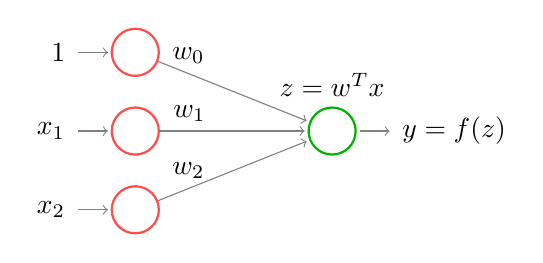
\begin{tikzpicture}[shorten >=1pt,->,draw=black!50, node distance=2.5cm]
    \tikzstyle{every pin edge}=[<-,shorten <=1pt]
    \tikzstyle{neuron}=[circle,minimum size=17pt,inner sep=0pt, line width=0.8]
    \tikzstyle{input neuron}=[neuron, draw=red!70];
    \tikzstyle{output neuron}=[neuron, draw=green!70!black];
    \tikzstyle{hidden neuron}=[neuron, draw=blue!65];
    \tikzstyle{annot} = [text width=4em, text centered]


    % Draw the input layer nodes
    \node[input neuron, pin=left: $1$] (I-0) at (0,0cm) {};
    \foreach \name / \y in {1,...,2}
      \node[input neuron, pin=left: $x_\y$] (I-\name) at (0,-\y cm) {};

    % Draw the output layer node
      \node[output neuron, pin={[pin edge={->,shorten <=1pt}]right: $y = f(z)$}, label={above:$z = w^Tx$}] (O-1) at (2.5cm,-1cm) {};

    \foreach \source in {0,...,2}
            \path (I-\source) edge node[above,pos=.2]{$w_\source$} (O-1);
\end{tikzpicture}
